\chapter{Overview of the Logistics of HYPERION}

\section{Methodology of Simulation}

For this simulation, we import a model array using the AIPy AntennaArray 
framework, which enables us to carry around an array with known geometry and 
baseline separations, along with individual antenna beam patterns and 
accessible frequencies. With this information and the previously made sky maps, 
we are now able to calculate our visibilities across many frequencies by using 
Eq.~\eqref{eq:vis}.

The AntennaArray framework also enables us to carry around models of the beams 
of the antennas, which is a convenient way to import absorbers into the 
simulation. Essentially, within the context of the simulation, the absorbers 
act as a modification term on the beam pattern, changing the way that each 
individual antenna sees the sky. This works as follows:

To start, we need a beam. HYPERION uses SARAS-style fat dipole antennas in our 
instrument, which means we will be using a frequency-invariant dipole beam 
pattern in our simulation to match~\citep{patra2013}. This is the base beam 
model used throughout the simulation, calculated using 
Eq.~\eqref{eq:dipole-beam}.

\begin{equation}
    \label{eq:dipole-beam}
    A(\theta, \phi, \nu) = \cos\Big(\frac{\frac{\pi}{2} 
    \cos{\theta}}{\sin{\theta}}\Big)
\end{equation}

The parameters we can play with are the absorptivity of the material (i.e. how 
much attenuation does the absorber provide at each frequency), the height of 
the absorber walls, and how smooth the transition from absorber to sky is.  

\section{Absorber Baffles -- Initial Results}

TALK ABOUT SYSTEM TEMPERATURE, NO NEED TO COOL BAFFLES (memo 1)

To date, we are still relatively early in the testing of our hypothesis that 
absorber walls or ``baffles" between antennas will enable us to better observe 
the spatial monopole with an interferometer. There have been two main sets of 
tests performed so far -- one in-lab test to measure the absorptivity of 
various proposed materials, and some brief field tests to gauge the 
effectiveness of our absorber at mitigating cross-talk between antennas.

The in-lab test was, in essence, a simple antenna return-loss measurement. To 
conduct the measurements, we started by constructing a large (i.e. 4.5' cube) 
Faraday cage out of wood and chicken wire, and placed an antenna at its center.  
From this setup, we could perform a simple return loss measurement and see what 
the maximum power return to the antenna is.

We could then line the cage with various absorptive materials and take another 
return-loss measurement, this time with (ideally) much of the power absorbed by 
the absorber, and see how effective each material is at dissipating energy 
within our science band. One such measurement is shown in 
Fig.~\ref{fig:fe-absorption}, featuring our most promising absorber candidate 
material, ferrite tiles.

\begin{figure}
    \begin{center}
    \includegraphics[width=\linewidth]{fe_absorption.png}
    \end{center}
    \caption{
        Here we see the results of a closed-box return loss measurement taken 
        with a densely packed (i.e. $9\times9$ tiles per wall) configuration of 
        ferrite tiles, evenly spaced along the walls of the testing Faraday 
        cage. The ripples are an artifact from the testing setup, and not 
        inherent to the performance of the ferrite itself. As can be easily 
        seen, the Ferrite performs much better at the high range of our science 
        band, and is optimized around $\sim120$ MHz.  While this material has 
        the best performance out of all the materials we have looked into so 
        far, we would ideally prefer a material with a more even absorptivity 
        across the band, so as best to avoid inadvertently adding ripples or 
        structure to our sky observations.
    }
    \label{fig:fe-absorption}
\end{figure}

As can be easily seen in the figure, the ferrite tiles have a decent 
absorptivity profile across the band, and an excellent absorptivity around 120 
MHz. However, as described in Section~\ref{sec:global-signal-overview}, the 
global signal of reionization is rich with physical information that is 
uniquely tied to its changing amplitude by frequency. The kinds of variations 
that we see in the absorptivity across the band are dangerous for the 
well-being of our experiment, as they could translate to tricky or uncertain 
calibration of our final instrument. We want to ensure that almost everything 
beyond the global signal has simple and well-defined relations to frequency 
(e.g. the synchrotron galactic sky, which is well described by a power law), in 
order to best understand our signal and be sure that instrumental 
idiosyncracies aren't being mistaken for true signal and science. As such, we 
would strongly prefer an absorber (or combination of absorbers) that has a more 
uniform performance across the science band.

Additionally, the ferrite tiles are among the most expensive of the materials 
we investigated. Even with a very close spacing and therefore relatively small 
baffle structures, the costs of acquiring enough ferrite to create an array 
quickly becomes overwhelming to the budget.
%\footnote{Of course, there's no longer any need to worry about that because 
%there is no budget -- this project dies alongside my academic ideals.}.

Other candidate absorbers include mats of Zotefoam Plastazote\textregistered, 
the AEP-EM low-frequency pyramidal foam absorber from DJM Electronics, and the 
creation of a grid of resistors designed to match with the free-space 
impedance~\citep{mahesh2015}. The Zotefoam was appealing due to its low cost 
compared to the pyramidal foam and ferrite tiles, but unfortunately its 
performance seemed to scale in proportion to its price tag.  The pyramidal foam 
performed slightly better, but seemed to feature more reflections than the 
ferrite and overall had a lower absorptivity performance than the ferrite, 
despite a nearly identical price tag per square foot of coverage. The resistive 
mesh is still an attractive idea, as it would only cost us an ungodly amount of 
effort to put together and about \$10 worth of resistors. Unfortunately, at the 
time of writing, only a very introductory level of investigation has been put 
into the resistive mesh idea, so nothing conclusive can be said about its 
performance as an absorber material.

At this point in time, there really haven't been any meaningful field tests 
upon which I could report. However, the most important things for us to 
investigate in the field would be a) ability of the absorber to mitigate the 
cross-talk between antennas and b) the efficacy of the baffles' ability to 
impose a spatial temperature variation from the antenna's point-of-view and how 
that efficacy evolves over frequency.

In Fig.~\ref{fig:field-test}, we see one possible arrangement of the absorber 
materials in order to assess the ability of the absorber at mitigating 
cross-talk between antennas. In order to perform this test adequately, one 
would need to take two measurements in the same radio environment -- one 
without the absorber between the antennas, in order to gauge the baseline level 
of cross-talk, and one with the absorber between, to measure the improvement in 
power leakage.

\begin{figure}
    \begin{center}
    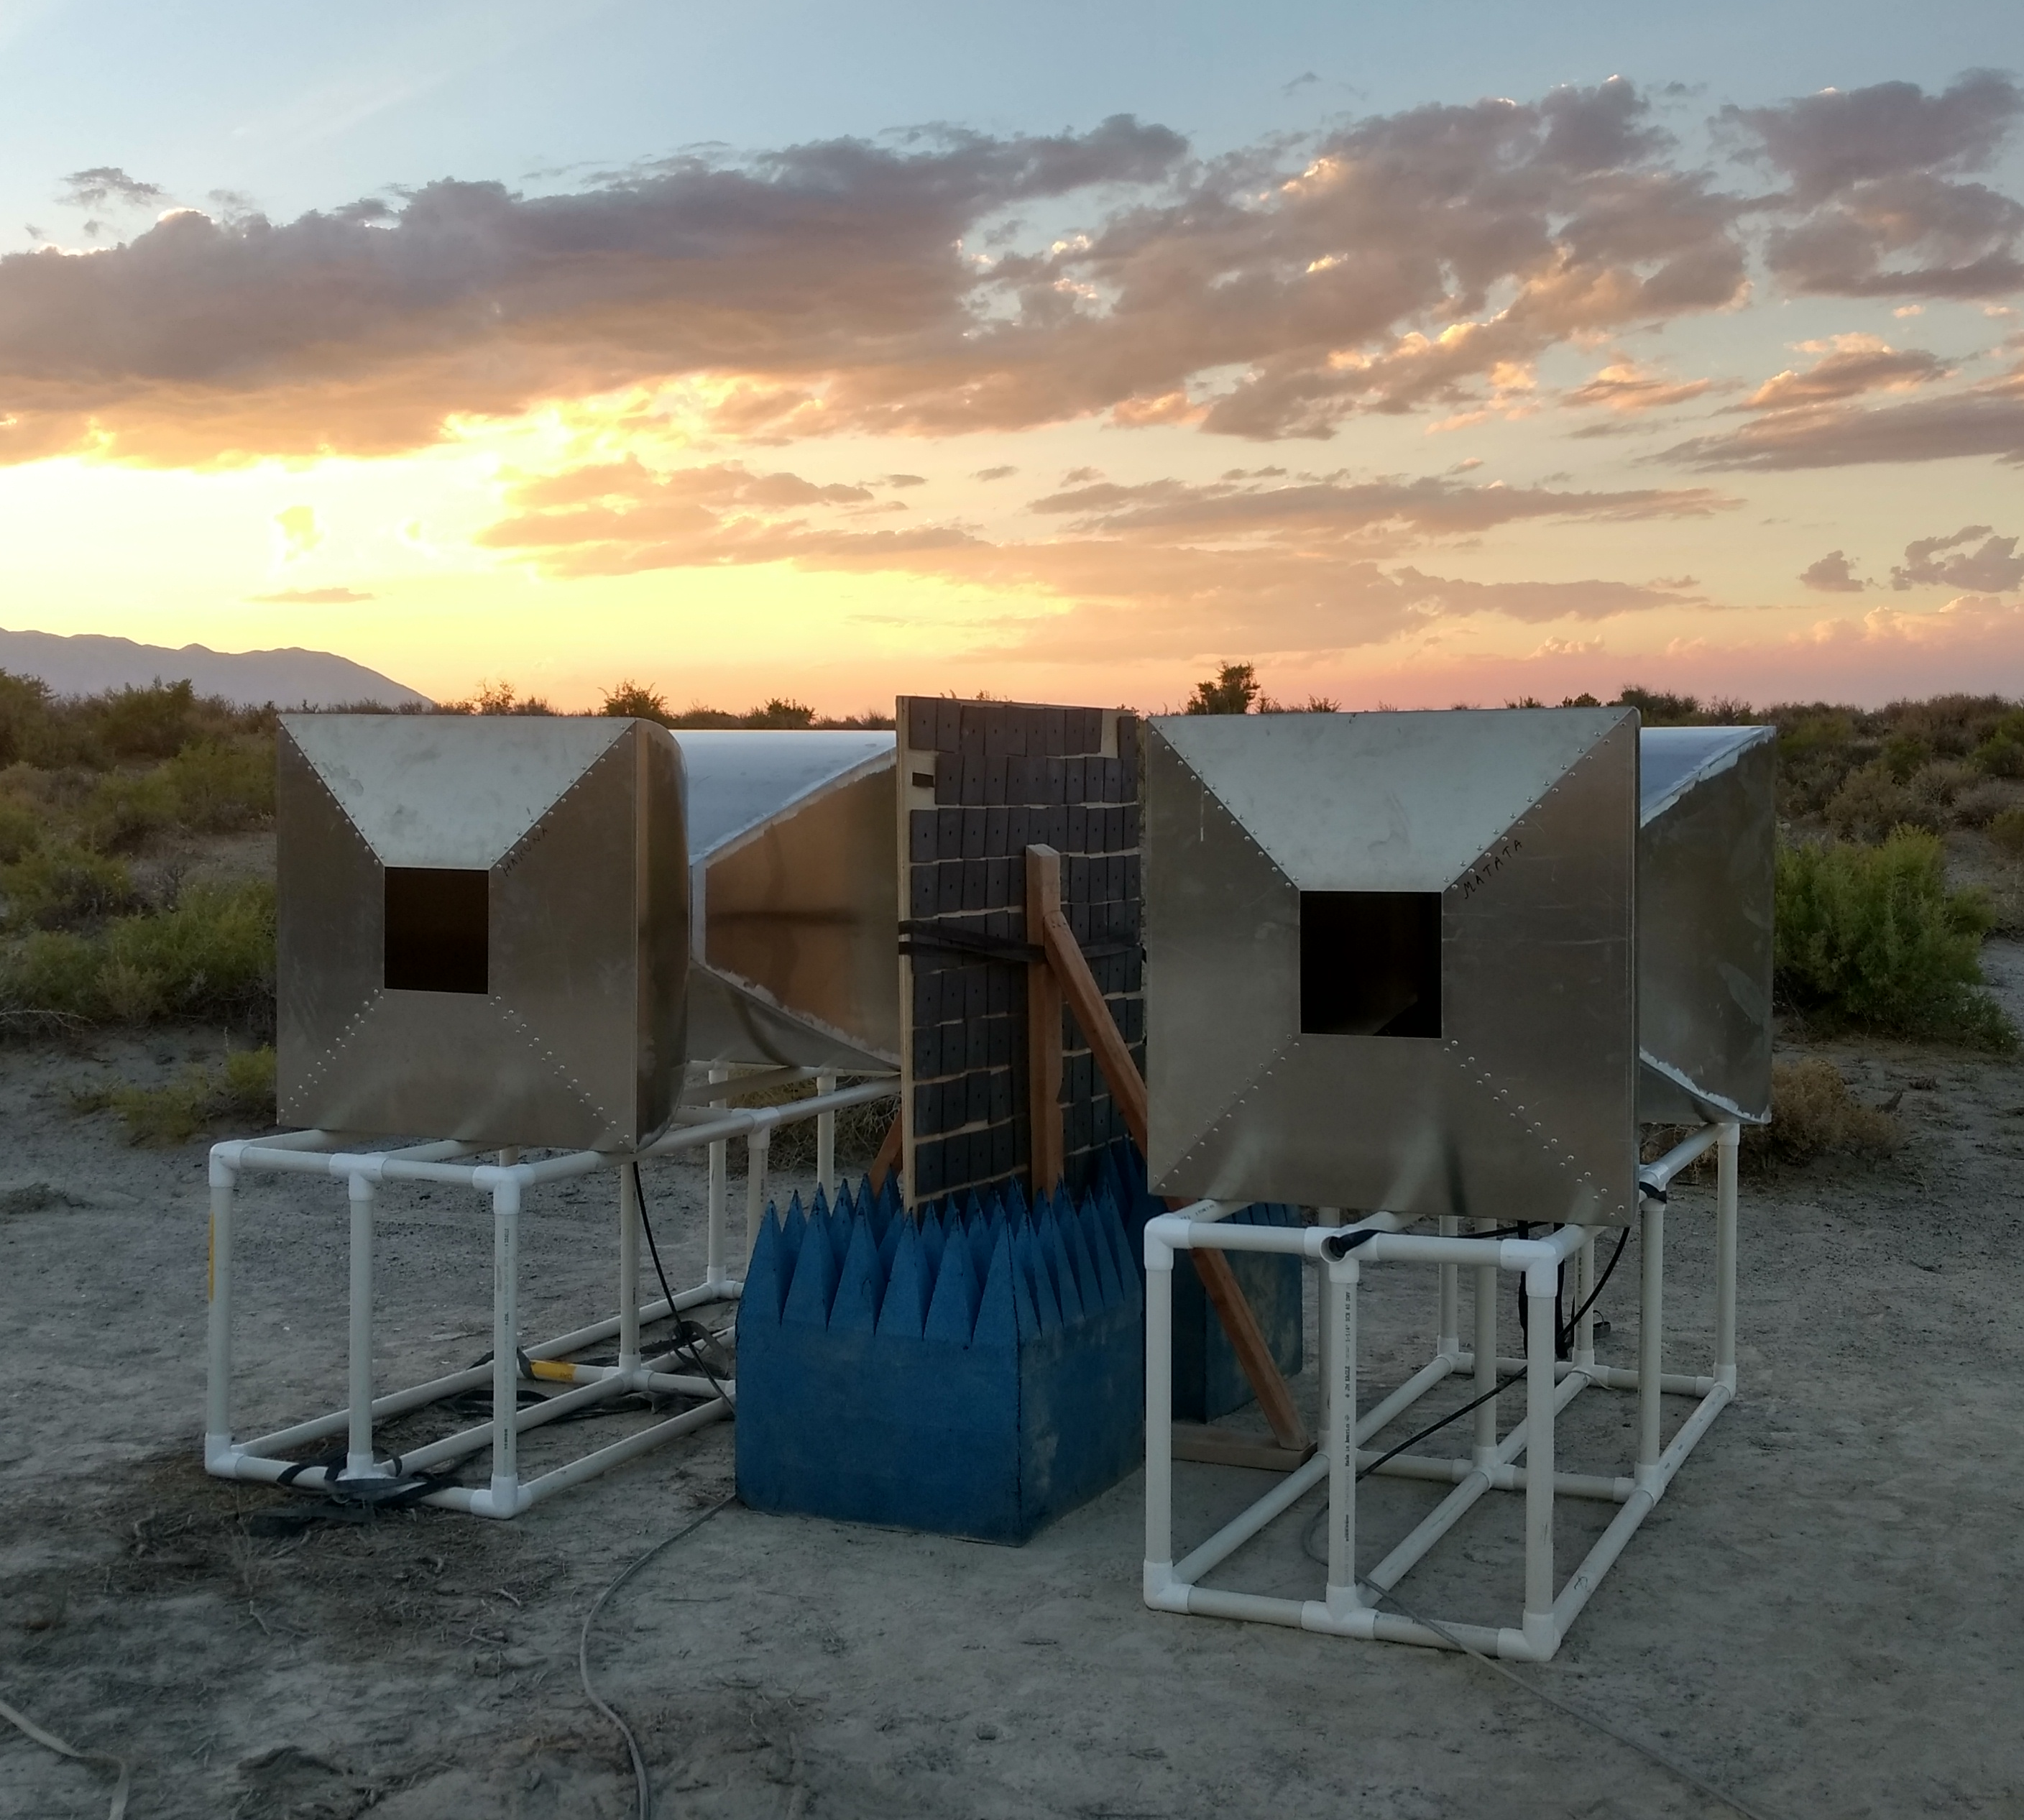
\includegraphics[width=\linewidth]{field-test.png}
    \end{center}
    \caption{
        Shown here is a simple diagnostic field set-up that could be used to 
        evaluate an absorber's ability to mitigate cross-talk between elements.  
        Here we used a densely-packed configuration of ferrite tiles that have 
        been propped up on some of our pyramidal foam absorber for additional 
        height.
    }
    \label{fig:field-test}
\end{figure}
